\section{Continuous-Time Fourier Series}

\subsection{Introduction}
\begin{frame}{Introduction}
    \begin{itemize}[<+->]
      \item Using the Fourier techniques we can obtain the frequency-domain representation of signals.
      \item We use Fourier series for periodic signals, and Fourier transform for aperiodic signals.
      \item Each of these have continuous-time and discrete-time versions:
        \begin{enumerate}
            \item Continuous-time Fourier series
            \item Continuous-time Fourier transform
            \item Discrete-time Fourier series
            \item Discrete-time Fourier transform
        \end{enumerate}
      \item In this part of the course, we will concentrate on how to actually compute continuous-time Fourier series and transform. Later, after we study liner, time-invariant (LTI) systems, we will study the conceptual aspects of Fourier techniques.
    \end{itemize}
\end{frame}

\begin{frame}
    \begin{columns}[t]
        \begin{column}{0.4\textwidth}
            \begin{figure}
              \centering
              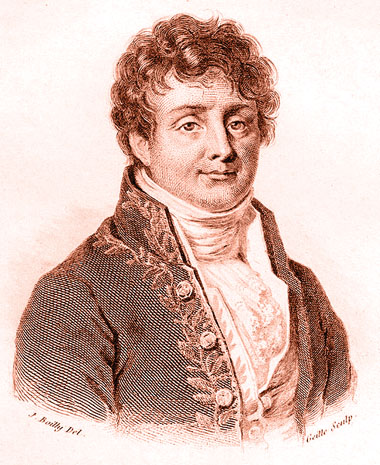
\includegraphics[width=0.4\textwidth]{figures/fourier.jpg}
              \caption{Jean-Baptiste Joseph Fourier, 1768--1830, French mathematician who discovered Fourier series and transform}\label{fi:secb_fourier}
            \end{figure}
        \end{column}
        \begin{column}{0.6\textwidth}
            \begin{itemize}[<+->]
              \item Every signal has a frequency distribution or a \alert{spectrum}.
              \item Periodic signals have a line spectra, called the Fourier series.
              \item The French mathematician, Jean-Baptiste Joseph Fourier, discovered this representation.
              \item Fourier series provides a way  to represent a periodic signal as a sum of complex exponentials.
              \item These sinusoids will be at frequencies that are integer multiples of the fundamental frequency $\omega_0$.
              \item $\omega_0 = \frac{2\pi}{T}$, where $T$: fundamental period of the waveform.
            \end{itemize}
        \end{column}
    \end{columns}
\end{frame}

\subsection{Fourier Series}

\begin{frame}{Continuous-Time Fourier Series}
    \mode<beamer>
    {
        \begin{equation}\label{eq:secb_fourierseries}
            \begin{aligned}
                x(t) &= \sum_{k=-\infty}^{+\infty}a_k e^{jk\omega_0 t}\\
                a_k &= \frac{1}{T} \int_{T}x(t)e^{-jk\omega_0 t}dt\\
                \omega_0 &= \frac{2\pi}{T}
            \end{aligned}
        \end{equation}
        The set of coefficients $\left\{a_k\right\}$ is called the \alert{Fourier series coefficients} or the \alert{spectral coefficients} of $x(t)$.
        The coefficient $a_0$ is the dc or constant component of $x(t)$, given by Equation \ref{eq:secb_fourierseries} with $k=0$:
        \begin{equation}\label{eq:secb_a0}
            a_0 = \frac{1}{T} \int_{T}x(t)dt,
        \end{equation}
        which is simply the average of $x(t)$ over one period.
    }
\end{frame}

\begin{frame}[plain]
    \begin{example}
        Let
        \begin{equation*}
            x(t) = \sin \omega_0t,
        \end{equation*}
        which has the fundamental frequency $\omega_0$.
    \end{example}
    \pause
    \begin{tikzpicture}[remember picture,overlay]
        \node[draw=red!50, fill=red!10, inner sep=2pt,outer sep=2pt, rounded corners=0.1cm, anchor=south east, yshift=7cm, xshift=-1cm, text width=3cm, align=left]  at (current page.south east) {Euler's formula\\$e^{j\theta} = \cos\theta + j\sin\theta$\\$\sin \theta = \frac{e^{j\theta} - e^{-j\theta}}{2j}$} ;
    \end{tikzpicture}
    \pause
    \mode<beamer>
    {
        \begin{equation*}
            \sin \omega_0t = \frac{1}{2j}e^{j\omega_0 t}- \frac{1}{2j}e^{-j\omega_0 t}
        \end{equation*}
        Comparing the right-hand side of this equation and Equation \ref{eq:secb_fourierseries}, we obtain
        \begin{equation*}
            \begin{split}
            a_1 &=  \frac{1}{2j} \qquad a_{-1} = -\frac{1}{2j}\\
            a_k &=0, \qquad k \neq \pm 1.\\
            \end{split}
        \end{equation*}
    }
\end{frame}

\begin{frame}[plain]
    \begin{example}
        Let
        \begin{equation*}
            x(t) = 1 + \sin \omega_0t + 2\cos\omega_0t+ \cos\left(2\omega_0t+ \frac{\pi}{4}\right),
        \end{equation*}
        which has the fundamental frequency $\omega_0$.
        \begin{enumerate}
            \item Use Euler's formula to express $x(t)$ as a liner combination of complex exponentials.
            \item Find the Fourier series coefficients, $a_k$.
            \item Plot the magnitude and phase of $a_k$.
        \end{enumerate}

    \end{example}
\end{frame}

\begin{frame}<beamer>[plain,t]
        \begin{equation*}
            x(t) = 1 + \sin \omega_0t + 2\cos\omega_0t+ \cos\left(2\omega_0t+ \frac{\pi}{4}\right),
        \end{equation*}

        \begin{tikzpicture}[remember picture,overlay]
          \node[draw=blue!50, fill=blue!20, inner sep=2pt,outer sep=2pt, rounded corners=0.1cm, anchor=south east, yshift=6.5cm, xshift=0cm, text width=3cm, align=left]  at (current page.south east) {Euler's formula\\$e^{j\theta} = \cos\theta + j\sin\theta$\\$\cos \theta = \frac{e^{j\theta} + e^{-j\theta}}{2}$\\$\sin \theta = \frac{e^{j\theta} - e^{-j\theta}}{2j}$} ;
        \end{tikzpicture}

        Using Euler's formula
        \begin{equation*}
            x(t) = 1 + \frac{1}{2j}\left[e^{j\omega_0 t} - e^{-j\omega_0 t}\right] + \left[e^{j\omega_0 t} + e^{-j\omega_0 t}\right] + \frac{1}{2}\left[e^{j(2\omega_0 t + \pi/4)} + e^{-j(2\omega_0 t + \pi/4)}\right]
        \end{equation*}
        \pause
        Collecting terms,
        \begin{equation*}
            x(t) = 1 + \left(1 + \frac{1}{2j}\right)e^{j\omega_0 t} +  \left(1 - \frac{1}{2j}\right)e^{-j\omega_0 t} + \left(\frac{1}{2} e^{j\pi/4}\right)e^{j2\omega_0 t} + \left(\frac{1}{2} e^{-j\pi/4}\right)e^{-j2\omega_0 t}
        \end{equation*}
        \pause
        \begin{columns}
            \begin{column}{0.5\textwidth}
                The Fourier coefficients are
                \begin{equation*}
                    \begin{split}
                        a_0 &= 1,\\
                        a_1 &= \left(1 + \frac{1}{2j}\right) = \left(1 - \frac{j}{2}\right),\\
                        a_{-1} &= \left(1 - \frac{1}{2j}\right) = \left(1 + \frac{j}{2}\right),\\
                    \end{split}
                \end{equation*}
            \end{column}
            \begin{column}{0.5\textwidth}
                \begin{equation*}
                    \begin{split}
                        a_2 &= \frac{1}{2}e^{j\pi/4} = \frac{\sqrt{2}}{4}(1+j),\\
                        a_{-2} &= \frac{1}{2}e^{-j\pi/4} = \frac{\sqrt{2}}{4}(1-j),\\
                        a_k &= 0, |k|>2.
                    \end{split}
                \end{equation*}
            \end{column}
        \end{columns}

\end{frame}

\begin{frame}<beamer>[plain,t]
    \begin{figure}
      \centering
      \begin{tikzpicture}
	\def\w{{-3, -2, -1,0,1, 2, 3}}
	\def\akmag{{0, 0.5, 1.1180,  1, 1.1180, 0.5, 0}}
	\def\akarg{{0, -0.7854, 0.4636, 0, -0.4636, 0.7854, 0}}

	\begin{scope}	
		\draw (-4, 0) -- (4,0) node[anchor=west] {\small $k$};
		\foreach \k in {-3,-2, ..., 3}
		{
			\node at (\k, 0) [anchor=north] {\small $\k$};
		}
		\node at (0,1.5) [anchor=south] {\small $|a_k|$};
		
		\foreach \k in {0,1, 2, 3, 4,5,6}
		{
			\pgfmathparse{\w[\k]}
			\edef\wk{\pgfmathresult}
			\pgfmathparse{\akmag[\k]}
			\edef\akmagk{\pgfmathresult}	
			\draw[thick] (\wk, 0) -- ++(0,\akmagk) node [anchor=south] {\small $\akmagk$};
			\ifthenelse{\lengthtest{0 pt = \akmagk pt}}{\draw[fill=black]  (\wk,0) circle (2pt);}{}
		}
	\end{scope}

	\begin{scope}[yshift=-1in]
		\draw (-4, 0) -- (4,0) node[anchor=west] {\small $k$};
		\foreach \k in {0,1, ..., 6}
		{			
			\pgfmathparse{\w[\k]}
			\edef\wk{\pgfmathresult}
			\pgfmathparse{\akarg[\k]}
			\edef\akargk{\pgfmathresult}	
			\pgfmathint{\wk}
			\edef\km3int{\pgfmathresult}
			\pgfmathsign{\akargk}
            \def\argsign{\pgfmathresult}		
			%\ifthenelse{-1=\argsign}{\node at (\wk, 0) [anchor=south] {\small $\km3int$};}{\node at (\wk, 0) [anchor=north] {\small $\km3int$};}
			\ifthenelse{-1=\argsign}{\edef\anchor{north}}{\edef\anchor{south}}			
			\ifthenelse{-1=\argsign}{\edef\anchorr{south}}{\edef\anchorr{north}}	
			\draw[thick] (\wk, 0) -- ++(0,\akargk) node[anchor=\anchor] {\small $\akargk$};
			\path (\wk,0) node [anchor=\anchorr] {\small  $\wk$};
			\ifthenelse{\lengthtest{0 pt = \akargk pt}}{\draw[fill=black]  (\wk,0) circle (2pt);}{}			
		}
		\node at (0,1.2) [anchor=south] {\small $\sphericalangle a_k$};				
	\end{scope}
\end{tikzpicture} 
      \caption{$|a_k|$, $\sphericalangle a_k$}\label{fi:secb-example01_fourier_euler}
    \end{figure}
\end{frame}



\begin{frame}
    \begin{example}
        The periodic square wave, sketched below, is defined over one period as
        \begin{equation*}
            x(t) = \begin{cases}
                1, & |t| <T_1,\\
                0, & T_1 < |t| < T/2,
            \end{cases}
        \end{equation*}
        This signal is periodic with fundamental period $T$ and fundamental frequency $\omega_0 = 2\pi/T$.
        \begin{enumerate}
            \item Find the Fourier series coefficients, $a_k$.
            \item Plot the magnitude and phase of $a_k$ for the case $T=4T_1$.
        \end{enumerate}
    \end{example}

%\end{frame}

%\begin{frame}[plain,t]
    \mode<beamer>
    {
        \begin{figure}
          \centering
          \begin{tikzpicture}[scale=0.9]
	\def\xmin{-7}
	\def\xmax{7}
	\def\ymin{0}
	\def\ymax{2}
	\def\period{2.0}
	\def\T1{0.3}
	\def\A{1}
	
	\edef\pulse{|- ++(2*\T1, \A) |- ++( \period - \T1, -\A)}

	
	\draw (\xmin-1, 0) --(\xmax+1, 0) node[anchor=west] {\small $t$};
	\draw (0, \ymin) --(0, \ymax) node[anchor=south] {\small $x(t)$};
		\foreach \x in {-3, -2, ..., 3}
		{
			\pgfmathmultiply{\period}{\x}
			\edef\position{\pgfmathresult}
			\ifthenelse{\NOT \x=0}
			{
				\node at (\position, 0) [anchor=north] {\small $\x T$};
			}
			{
				%\node at (\position, 0) [anchor=north] {\small $0$};
			}
			\draw (\position-\T1, 0) \pulse;	
			\draw (\position, 0) -- ++(0,0.1);
			%\pulse{3}{0.4};		
		}
		
		\node at (-\T1, 0) [anchor=north] {\small $-T_1$};
		\node at (\T1, 0) [anchor=north] {\small $T_1$};
		\node at (-\period/2, 0) [anchor=north] {\small $-\frac{T}{2}$};
		\node at (\period/2, 0) [anchor=north] {\small $\frac{T}{2}$};
		\draw (-\period/2, 0) -- ++(0,0.1);
		\draw (\period/2, 0) -- ++(0,0.1);

		\node at (\xmin, \A/2) {$\dots$};
		\node at (\xmax, \A/2) {$\dots$};
\end{tikzpicture}

          \caption{Periodic square wave}\label{fi:example02_periodic_square_wave }
        \end{figure}
    }
\end{frame}

\begin{frame}
    \mode<beamer>
    {
        \begin{columns}
          \begin{column}{0.5\textwidth}
                \begin{equation*}
                    \begin{split}
                       a_0 &= \frac{1}{T} \int_{T}x(t)dt,\\
                       &=  \frac{1}{T} \int_{-T_1}^{T_1}1dt,\\
                       &= \frac{2T_1}{T}.
                    \end{split}
                \end{equation*}
                \pause
                \begin{equation*}
                    \begin{split}
                       a_k &= \frac{1}{T} \int_{T}x(t)e^{-jk\omega_0 t}dt,\\
                       &=  \frac{1}{T} \int_{-T_1}^{T_1}e^{-jk\omega_0 t}dt,\\
                       &= -\left. \frac{1}{jk\omega_0 T}e^{-jk\omega_0 t}\right|^{T_1}_{-T_1}
                    \end{split}
                \end{equation*}
          \end{column}
          \begin{column}{0.5\textwidth}
                \pause

            \begin{tikzpicture}[remember picture,overlay]
              \node[draw=blue!50, fill=blue!20, inner sep=2pt,outer sep=2pt, rounded corners=0.1cm, anchor=south east, yshift=1cm, xshift=-1cm, text width=3cm, align=left]  at (current page.south east) {Euler's formula\\$e^{j\theta} = \cos\theta + j\sin\theta$\\$\cos \theta = \frac{e^{j\theta} + e^{-j\theta}}{2}$\\$\sin \theta = \frac{e^{j\theta} - e^{-j\theta}}{2j}$} ;
            \end{tikzpicture}
                \pause

                \begin{equation*}
                    \begin{split}
                       a_k &= \frac{2}{k\omega_0 T}\left[\frac{e^{jk\omega_0 T_1} - e^{-jk\omega_0 T_1}}{2j}\right]\\
                       a_k &= \frac{2\sin(k\omega_0 T_1)}{k\omega_0 T} = \frac{\sin(k\omega_0 T_1)}{k\pi}, k \neq 0.
                    \end{split}
                \end{equation*}
          \end{column}
        \end{columns}


    }
\end{frame}

\begin{frame}
    \mode<beamer>
    {
    For $T=4T_1$
    \begin{equation*}
        a_k = 0, \quad k \text{ even}.
    \end{equation*}
    \begin{align*}
        a_0 &= \frac{1}{2}\\
        a_1 &= a_{-1} = \frac{1}{\pi}\\
        a_3 &= a_{-3} = -\frac{1}{3\pi}\\
        a_5 &= a_{-5} = \frac{1}{5\pi}\\
    \end{align*}
    }
\end{frame}


\begin{frame}<beamer>[plain,t]
    \begin{figure}
      \centering
      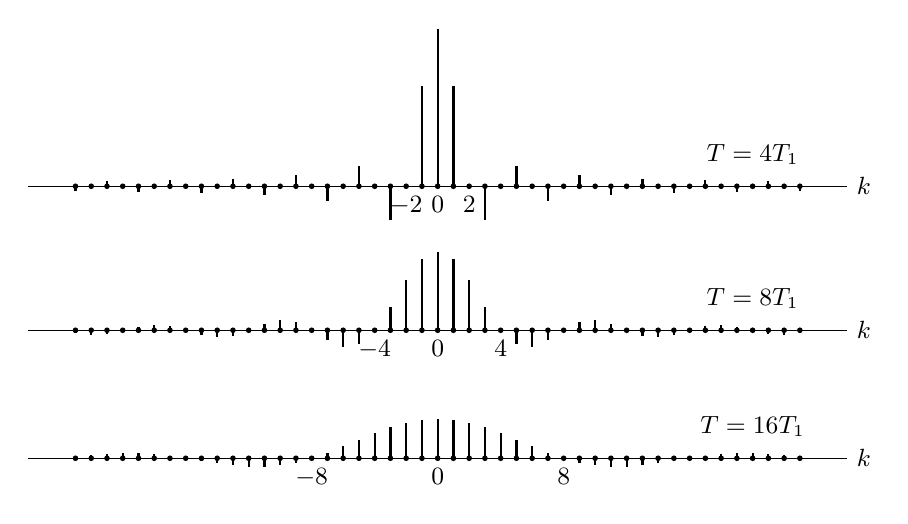
\begin{tikzpicture}[scale=0.4]
	\def\w{{-23,-22,-21,-20,-19,-18,-17,-16,-15,-14,-13,-12,-11,-10,-9,-8,-7,-6,-5,-4,-3,-2,-1,0,1,2,3,4,5,6,7,8,9,10,11,12,13,14,15,16,17,18,19,20,21,22,23}}
	\def\akmag{{-0.013840,0.000000,0.015158,-0.000000,-0.016753,0.000000,0.018724,-0.000000,-0.021221,0.000000,0.024485,-0.000000,-0.028937,0.000000,0.035368,-0.000000,-0.045473,0.000000,0.063662,-0.000000,-0.106103,0.000000,0.318310,0.500000,0.318310,0.000000,-0.106103,-0.000000,0.063662,0.000000,-0.045473,-0.000000,0.035368,0.000000,-0.028937,-0.000000,0.024485,0.000000,-0.021221,-0.000000,0.018724,0.000000,-0.016753,-0.000000,0.015158,0.000000,-0.013840}}


	\begin{scope}	
		\draw (-13, 0) -- (13,0) node[anchor=west] {\small $k$};
		\foreach \k in {-2, 0, 2}
		{
			\node at (\k/2, 0) [anchor=north] {\small $\k$};
		}
		%\node at (0,5) [anchor=south] {\small $Ta_k$};
		
		\foreach \k in {0,1, ..., 46}
		{
			\pgfmathparse{\w[\k]/2}
			\edef\wk{\pgfmathresult}
			\pgfmathparse{\akmag[\k]}
			\edef\akmagk{\pgfmathresult}	
			\draw[thick] (\wk, 0) -- ++(0,10*\akmagk);% node [anchor=south] {\small $\akmagk$};
			\ifthenelse{\lengthtest{0 pt = \akmagk pt}}{\draw[fill=black]  (\wk,0) circle (2pt);}{}
		}
			\node at (10, 1) {\small $T= 4T_1$};		
	\end{scope}


\def\akmag{{-0.009786,-0.014469,-0.010718,0.000000,0.011846,0.017684,0.013240,-0.000000,-0.015005,-0.022736,-0.017314,0.000000,0.020462,0.031831,0.025009,-0.000000,-0.032154,-0.053052,-0.045016,0.000000,0.075026,0.159155,0.225079,0.250000,0.225079,0.159155,0.075026,0.000000,-0.045016,-0.053052,-0.032154,-0.000000,0.025009,0.031831,0.020462,0.000000,-0.017314,-0.022736,-0.015005,-0.000000,0.013240,0.017684,0.011846,0.000000,-0.010718,-0.014469,-0.009786}}


	\begin{scope}[yshift=-1.8in]
		\draw (-13, 0) -- (13,0) node[anchor=west] {\small $k$};
		\foreach \k in {-4, 0, 4}
		{
			\node at (\k/2, 0) [anchor=north] {\small $\k$};
		}
		%\node at (0,5) [anchor=south] {\small $Ta_k$};
		
		\foreach \k in {0,1, ..., 46}
		{
			\pgfmathparse{\w[\k]/2}
			\edef\wk{\pgfmathresult}
			\pgfmathparse{\akmag[\k]}
			\edef\akmagk{\pgfmathresult}	
			\draw[thick] (\wk, 0) -- ++(0,10*\akmagk);% node [anchor=south] {\small $\akmagk$};
			\ifthenelse{\lengthtest{0 pt = \akmagk pt}}{\draw[fill=black]  (\wk,0) circle (2pt);}{}		
		}
			\node at (10, 1) {\small $T= 8T_1$};			
	\end{scope}

\def\akmag{{0.005296,0.010231,0.014004,0.015915,0.015478,0.012504,0.007165,-0.000000,-0.008121,-0.016077,-0.022622,-0.026526,-0.026735,-0.022508,-0.013535,0.000000,0.017402,0.037513,0.058816,0.079577,0.098027,0.112540,0.121812,0.125000,0.121812,0.112540,0.098027,0.079577,0.058816,0.037513,0.017402,0.000000,-0.013535,-0.022508,-0.026735,-0.026526,-0.022622,-0.016077,-0.008121,-0.000000,0.007165,0.012504,0.015478,0.015915,0.014004,0.010231,0.005296}}


	\begin{scope}[yshift=-3.4in]
		\draw (-13, 0) -- (13,0) node[anchor=west] {\small $k$};
		\foreach \k in {-8, 0, 8}
		{
			\node at (\k/2, 0) [anchor=north] {\small $\k$};
		}
		%\node at (0,5) [anchor=south] {\small $Ta_k$};
		
		\foreach \k in {0,1, ..., 46}
		{
			\pgfmathparse{\w[\k]/2}
			\edef\wk{\pgfmathresult}
			\pgfmathparse{\akmag[\k]}
			\edef\akmagk{\pgfmathresult}	
			\draw[thick] (\wk, 0) -- ++(0,10*\akmagk);% node [anchor=south] {\small $\akmagk$};
			\ifthenelse{\lengthtest{0 pt = \akmagk pt}}{\draw[fill=black]  (\wk,0) circle (2pt);}{}
		}
			\node at (10, 1) {\small $T= 16T_1$};			
	\end{scope}

% 	\begin{scope}[yshift=-1in]
% 		\draw (-4, 0) -- (4,0) node[anchor=west] {\small $k$};
% 		\foreach \k in {0,1, ..., 6}
% 		{			
% 			\pgfmathparse{\w[\k]}
% 			\edef\wk{\pgfmathresult}
% 			\pgfmathparse{\akarg[\k]}
% 			\edef\akargk{\pgfmathresult}	
% 			\pgfmathint{\wk}
% 			\edef\km3int{\pgfmathresult}
% 			\pgfmathsign{\akargk}
%             \def\argsign{\pgfmathresult}		
% 			\ifthenelse{-1=\argsign}{\node at (\wk, 0) [anchor=south] {\small $\km3int$};}{\node at (\wk, 0) [anchor=north] {\small $\km3int$};}
% 			\ifthenelse{-1=\argsign}{\edef\anchor{north}}{\edef\anchor{south}}			
%
% 			\draw[thick] (\wk, 0) -- ++(0,\akargk) node[anchor=\anchor] {\small $\akargk$};;
% 			\ifthenelse{\lengthtest{0 pt = \akargk pt}}{\draw[fill=black]  (\wk,0) circle (2pt);}{}			
% 		}
% 		%\node at (0,1.2) [anchor=south] {\small $\sphericalangle a_k$};				
% 	\end{scope}
\end{tikzpicture} 
      \caption{Plots of scaled Fourier series coefficients $Ta_k$}\label{fi:example02_periodic_square_fs}
    \end{figure}
\end{frame}


\subsection{Properties of the Continuous-Time Fourier Series}

\begin{frame}
    Suppose that $x(t)$ is a periodic signal with period $T$ and fundamental frequency $\omega_0 = 2\pi/T$. Then if the Fourier series coefficients are denoted by $a_k$, then
    \begin{equation}
        x(t) \overset{\mathcal{FS}}{\longleftrightarrow} a_k
    \end{equation}
\end{frame}

\begin{frame}{Linearity}
    Let $x(t)$ and $y(t)$ denote two periodic signals with period $T$.
    \begin{align*}
        x(t) &\overset{\mathcal{FS}}{\longleftrightarrow} a_k,\\
        y(t) &\overset{\mathcal{FS}}{\longleftrightarrow} b_k.\\
    \end{align*}
    Any linear combination of the two signals will also be periodic with period $T$. Fourier series coefficients $c_k$ of the linear combination of $x(t)$ and $y(t)$, $z(t) = Ax(t) + By(t)$, are given by the same linear combination:
    \pause
    \mode<beamer>
    {
        \begin{equation}
            z(t) = Ax(t) + By(t)\overset{\mathcal{FS}}{\longleftrightarrow} c_k = Aa_k + Bb_k.
        \end{equation}
    }
\end{frame}

\begin{frame}[plain]{Time Shifting}
    \begin{equation}
        x(t-t_0) \overset{\mathcal{FS}}{\longleftrightarrow} e^{-jk\omega_0 t_0}a_k = e^{-jk(2\pi/T) t_0}a_k
    \end{equation}
    \mode<beamer>
    {
        \begin{tikzpicture}[remember picture,overlay]
            \node[draw=red!50, fill=red!10, inner sep=2pt,outer sep=2pt, rounded corners=0.1cm, anchor=south east, yshift=5cm, xshift=-1cm, text width=3cm, align=left]  at (current page.south east)
            {
                Fourier series:\\
                $x(t) = \sum_{k=-\infty}^{+\infty}a_k e^{jk\omega_0 t}$\par
                $a_k = \frac{1}{T} \int_{T}x(t)e^{-jk\omega_0 t}dt$

            } ;
        \end{tikzpicture}
        \noindent Proof:\\%Page 203
        \pause
        \begin{equation*}
            \begin{aligned}
          x(t) &\overset{\mathcal{FS}}{\longleftrightarrow} a_k, \quad x(t-t_0) \overset{\mathcal{FS}}{\longleftrightarrow} b_k,\\
                b_k &=  \frac{1}{T}\int_{T}x(t-t_0)e^{-jk\omega_0 t}dt,\\
                &= \frac{1}{T}\int_{T}x(\tau)e^{-jk\omega_0(\tau + t_0)}d\tau,\\
                &= e^{-jk\omega_0  t_0}\frac{1}{T}\int_{T}x(\tau)e^{-jk\omega_0\tau}d\tau,\\
                &= e^{-jk\omega_0  t_0}a_k.
            \end{aligned}
        \end{equation*}

        \begin{equation*}
             x(t-t_0) \overset{\mathcal{FS}}{\longleftrightarrow} e^{-jk\omega_0  t_0}a_k.
        \end{equation*}

        Note: $|a_k| = |b_k|$
    }
\end{frame}


\begin{frame}[plain]{Time Reversal}
    If
    \begin{equation*}
        x(t) \overset{\mathcal{FS}}{\longleftrightarrow} a_k
    \end{equation*}
    then
    \begin{equation*}
        x(-t) \overset{\mathcal{FS}}{\longleftrightarrow} a_{-k}.
    \end{equation*}
    \mode<beamer>
    {
        \begin{tikzpicture}[remember picture,overlay]
            \node[draw=red!50, fill=red!10, inner sep=2pt,outer sep=2pt, rounded corners=0.1cm, anchor=south east, yshift=5cm, xshift=-1cm, text width=3cm, align=left]  at (current page.south east)
            {
                Fourier series:\\
                $x(t) = \sum_{k=-\infty}^{+\infty}a_k e^{jk\omega_0 t}$\par
                $a_k = \frac{1}{T} \int_{T}x(t)e^{-jk\omega_0 t}dt$

            } ;
        \end{tikzpicture}

        \begin{equation*}
            x(-t) =  \sum_{k=-\infty}^{\infty}a_ke^{-jk2\pi t/T}.
        \end{equation*}
        Substitution: $k=-m$
        \begin{equation*}
            x(-t) = \sum_{m=-\infty}^{\infty}a_{-m}e^{jm2\pi t/T}.
        \end{equation*}
        %\pause
        Right-hand side of this equation has the form of the \fs synthesis equation for $x(-t)$, where the \fs coefficients  $b_k$ are
        \begin{equation*}
            b_k = a_{-k}.
        \end{equation*}

    }
\end{frame}

\begin{frame}<beamer>
    \begin{itemize}[<+->]
      \item Time reversal applied to a continuous-time signal results in a time reversal of the corresponding sequence of Fourier series coefficients.
      \item If $x(t)$ is even, i.e., $x(-t) = x(t)$, then its Fourier series coefficients are also even, i.e., $a_{-k}=a_k$.
      \item If $x(t)$ is odd, i.e., $x(-t) = -x(t)$, then its Fourier series coefficients are also odd, i.e., $a_{-k}=-a_k$.
    \end{itemize}
\end{frame}


\begin{frame}[plain]\frametitle{Time Scaling}
    Time scaling, in general, changes the period.\\
    If $x(t)$ is a periodic with period $T$ and fundamental frequency $\omega_0 = 2\pi/T$, then $x(\alpha t)$, where $\alpha$ is a positive real number, is periodic with period $T/\alpha$ and fundamental frequency $\alpha \omega_0$.
    \begin{equation}
        x(\alpha t) = \sum_{k=-\infty}^{\infty} a_k e^{jk(\alpha \omega_0)t}
    \end{equation}
    \mode<beamer>
    {

        While Fourier coefficients have not changes, the Fourier series representation \alert{has} changed because of the change in the fundamental frequency.

    }
\end{frame}


\begin{frame}[plain]\frametitle{Multiplication}
    \mode<beamer>
    {
        Let $x(t)$ and $y(t)$ denote two periodic signals with period $T$.
        \begin{align*}
            x(t) &\overset{\mathcal{FS}}{\longleftrightarrow} a_k,\\
            y(t) &\overset{\mathcal{FS}}{\longleftrightarrow} b_k.\\
        \end{align*}
        Since the product $x(t)y(t)$ is also periodic with period $T$, its Fourier series coefficients $h_k$ are
        \begin{equation}
            x(t)y(t) \overset{\mathcal{FS}}{\longleftrightarrow} h_k = \sum_{l=-\infty}^{\infty}a_l b_{k-l}.
        \end{equation}

    }
\end{frame}


\begin{frame}[plain]\frametitle{Conjugation and Conjugate Symmetry}
    %\mode<beamer>
    {

        \begin{itemize}[<+->]
          \item Taking the complex conjugate of a periodic signal $x(t)$ has the effect of complex conjugation and \alert{time reversal} on the corresponding Fourier series coefficients.
          \item If $x(t)$ is real, i.e., $x(t) = x^\ast(t)$: Fourier series coefficients conjugate symmetric, i.e., $a_{-k} = a^\ast_k$.
          \item If $x(t)$ is real, then $a_0$ is real and $|a_k| = |a_{-k}|$.
          \item If $x(t)$ is real and even, we know that $a_k = a_{-k}$. From above, $a^\ast_k = a_{-k}$, so that $a_{k} = a^\ast_k$. That is if $x(t)$ is real and even, so are its Fourier series coefficients.
          \item If $x(t)$ is real and odd, its Fourier series coefficients are purely imaginary and odd. Thus, e.g., $a_0 = 0$.% do probelm 3.42 in tutorial.
        \end{itemize}
    }
\end{frame}


\begin{frame}{Example}
    \begin{columns}
        \begin{column}{0.5\textwidth}
            Consider
            \begin{equation*}
                x_1(t) = \cos(\omega_0 t)
            \end{equation*}
            This is real and even.
            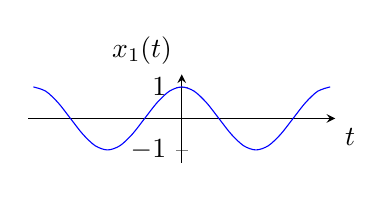
\begin{tikzpicture}[>=latex]
                \begin{axis}[
                    x = 0.3cm,
                    y = 0.4cm,
                    domain=-6.28:6.28,
                    smooth, no markers,
                    axis x line=center,
                    axis y line=center,
                    xlabel style={below right},
                    ylabel style={above left},
                    xlabel = {$t$},
                    ylabel = {$x_1(t)$},
                    xtick=\empty,
                    xmin=-6.5,
                    xmax=6.5,
                    ymin=-1.4,
                    ymax=1.4
                    ]
                    \addplot {cos(deg(x))};
                \end{axis}
            \end{tikzpicture}

            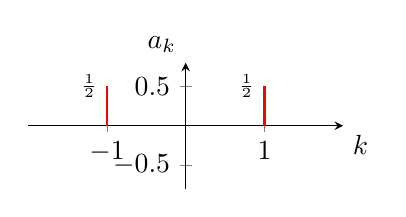
\begin{tikzpicture}
                \begin{axis}[
                    x = 1cm,
                    y = 1cm,
                    domain=-6.28:6.28,
                    smooth, no markers,
                    axis x line=center,
                    axis y line=center,
                    xlabel style={below right},
                    ylabel style={above left},
                    xlabel = {$k$},
                    ylabel = {$a_k$},
                    xtick={-1, 1},
                    xmin=-2,
                    xmax=2,
                    ymin=-0.8,
                    ymax=0.8
                    ]
                    \addplot+[ycomb, red, thick] coordinates {(-1,1/2) (1,1/2)};
                    \node at (axis cs:-1,1/2) [anchor=east] {\scriptsize $\frac{1}{2}$};
                    \node at (axis cs:1,1/2) [anchor=east] {\scriptsize $\frac{1}{2}$};
                \end{axis}
            \end{tikzpicture}

            FS coefficients are real and even. (They are conjugate symmetric too.)
        \end{column}
        \begin{column}{0.5\textwidth}
            Consider
            \begin{equation*}
                x_2(t) = \sin(\omega_0t)
            \end{equation*}
            This is real and odd.
            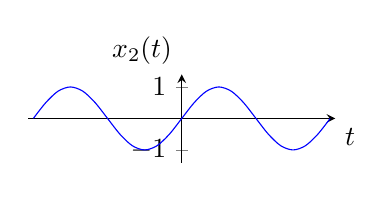
\begin{tikzpicture}[>=latex]
                \begin{axis}[
                    x = 0.3cm,
                    y = 0.4cm,
                    domain=-6.28:6.28,
                    smooth, no markers,
                    axis x line=center,
                    axis y line=center,
                    xlabel style={below right},
                    ylabel style={above left},
                    xlabel = {$t$},
                    ylabel = {$x_2(t)$},
                    xtick=\empty,
                    xmin=-6.5,
                    xmax=6.5,
                    ymin=-1.4,
                    ymax=1.4
                    ]
                    \addplot {sin(deg(x))};
                \end{axis}
            \end{tikzpicture}

            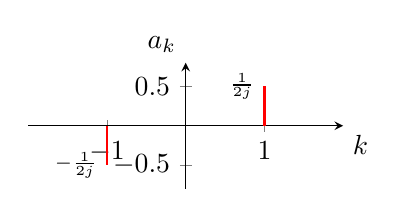
\begin{tikzpicture}
                \begin{axis}[
                    x = 1cm,
                    y = 1cm,
                    domain=-6.28:6.28,
                    smooth, no markers,
                    axis x line=center,
                    axis y line=center,
                    xlabel style={below right},
                    ylabel style={above left},
                    xlabel = {$k$},
                    ylabel = {$a_k$},
                    xtick={-1, 1},
                    xmin=-2,
                    xmax=2,
                    ymin=-0.8,
                    ymax=0.8
                    ]
                    \addplot+[ycomb, red, thick] coordinates {(-1,-1/2) (1,1/2)};
                    \node at (axis cs:-1,-1/2) [anchor=east] {\scriptsize $-\frac{1}{2j}$};
                    \node at (axis cs:1,1/2) [anchor=east] {\scriptsize $\frac{1}{2j}$};
                \end{axis}
            \end{tikzpicture}

            FS coefficients are imaginary and odd. (They are conjugate symmetric too.)
        \end{column}
    \end{columns}
\end{frame}


\begin{frame}\frametitle{Parseval's Relation for Continuous-Time Periodic Signals}
    \begin{equation}\label{eq:parseval}
        \frac{1}{T}\int_{T} |x(t)|^2dt = \sum_{k=-\infty}^{\infty}|a_k|^2.
    \end{equation}
    \pause
    \mode<beamer>
    {
        \noindent Note: Left-hand side of equation \ref{eq:parseval} is the average power (i.e., energy per unit time) in one period of the periodic signal $x(t)$.\\

        \begin{equation}
            \frac{1}{T}\int_{T} \left| a_k e^{jk\omega_0 t}\right|^2dt = \frac{1}{T}\int_{T} \left| a_k \right|^2dt = |a_k|^2.
        \end{equation}
        So, $|a_k|^2$ is the average power in the $k$th harmonic component of $x(k)$.\\
        Thus, what Parseval's relation states is that the total average power in a periodic signal equals the sum of the average powers in all of its harmonic components.
    }
\end{frame}

\begin{frame}
    \begin{example}%3.6
        Consider the signal $g(t)$ with a fundamental period of $4$, shown in Figure \ref{fi:example3p6}.
        \begin{figure}
          \centering
          \begin{tikzpicture}
	\draw (-4,0) -- (4,0) node [anchor=west] {\scriptsize $t$};
	\draw (0, -1) -- (0,1) node [anchor=south] {\scriptsize $g(t)$};
	\foreach \t in {-2, 2}
	{
		\draw (\t, 0.1) -- ++(0, -0.2) node[anchor=north, xshift=-1em] {\scriptsize $\t$}; 	
	}
	\foreach \t in {-1, 1}
	{
		\draw (\t, 0.1) -- ++(0, -0.2) node[anchor=north] {\scriptsize $\t$}; 
	
	}	
	
	\foreach \t in {0.5}
	{
		\draw (0.1, \t) -- ++(-0.2, 0) node[anchor=east] {\scriptsize $\t$}; 
	
	}	

	\foreach \t in {-0.5}
	{
		\draw (0.1, \t) -- ++(-0.2, 0) node[anchor=west, xshift=1em] {\scriptsize $\t$}; 
	
	}
	\draw[thick] (-3, 0.5) -| (-2, -0.5) -| (0,0.5) -| (2, -0.5) -- (3, -0.5);

\end{tikzpicture}
          \caption{Figure for example}\label{fi:example3p6}
        \end{figure}

        Determine the Fourier series representation of $g(t)$
        \begin{enumerate}
            \item directly from the analysis equation.
            \item by assuming that the Fourier series coefficients of the symmetric periodic square wave are known.
        \end{enumerate}
    \end{example}
\end{frame}



\begin{frame}{Solution: Direct}
 \mode<beamer>
{
    \begin{equation*}
        a_0 = 0, \quad a_k = \frac{1}{2\pi jk}\left(1-\cos k\pi\right)
    \end{equation*}
    \begin{equation*}
        a_1 = -j/\pi, a_2 = 0, a_3 = -j/(3\pi), a_4 = 0, a_5 = -j/(5\pi), \dots
    \end{equation*}
}
\end{frame}



\begin{frame}
\mode<beamer>
{
    \begin{columns}
        \column{0.5\textwidth}

            We notice that
            \begin{equation*}
                g(t) = x(t-1) - 1/2,
            \end{equation*}
            with $T=4$ and $T_1 = 1$.
            \pause
            If FS coefficients of $x(t)$ are denoted by $a_k$, the FS coefficients of $x(t-1)$ may be expressed as
            \begin{equation*}
                b_k = a_k e^{-jk\pi/2},
            \end{equation*}
            The FS coefficients of the dc offset $-1/2$
            \begin{equation*}
                c_k =
                \begin{cases}
                    0, & \text{for } k \neq 0,\\
                    -\frac{1}{2}& \text{for } k = 0.
                \end{cases}
            \end{equation*}
            \

        \column{0.5\textwidth}
            Applying the linearity property, the FS coefficients of $g(t)$ may be expressed as
            \pause
            \begin{equation*}
                d_k =
                \begin{cases}
                    a_k e^{-jk\pi/2}, & \text{for } k \neq 0,\\
                    a_0-\frac{1}{2}& \text{for } k = 0.
                \end{cases}
            \end{equation*}
            yielding
            \begin{equation*}
                d_k =
                \begin{cases}
                    \frac{\sin(\pi k/2)}{k\pi} e^{-jk\pi/2}, & \text{for } k \neq 0,\\
                    0& \text{for } k = 0.
                \end{cases}
            \end{equation*}
   \end{columns}
}
\end{frame}


\begin{frame}%3.7
    \begin{example}
        Consider the triangular wave signal $x(t)$ with period $T=4$ and fundamental frequency $\omega_0 = \pi/2$, shown in Figure \ref{fi:example3p7}. The derivative signal is the signal $g(t)$ in Figure \ref{fi:example3p6}. Using this information, find the Fourier series coefficients of $x(t)$.
        \begin{figure}
          \centering
          \begin{tikzpicture}
	\draw (-4,0) -- (4,0) node [anchor=west] {\scriptsize $t$};
	\draw (0, -0.2) -- (0,1.5) node [anchor=south] {\scriptsize $x(t)$};
	\foreach \t in {-2, 2}
	{
		\draw (\t, 0.1) -- ++(0, -0.2) node[anchor=north, xshift=-1em] {\scriptsize $\t$}; 	
	}
	\foreach \t in {-1, 1}
	{
		\draw (\t, 0.1) -- ++(0, -0.2) node[anchor=north] {\scriptsize $\t$};
	
	}	
	
	\foreach \t in {1}
	{
		\draw (0.1, \t) -- ++(-0.2, 0) node[anchor=east] {\scriptsize $\t$};
	
	}	


	\draw[thick] (-3, 0.5) -- (-2, 1) -- (0,0) -- (2, 1) -- (3, 0.5);

\end{tikzpicture} 
          \caption{Figure for example}\label{fi:example3p7}
        \end{figure}
    \end{example}
\end{frame}

\begin{frame}
\mode<beamer>
{
    The derivative of this signal is the signal $g(t)$ in the previous example. Denoting the Fourier coefficients of $g(t)$ by $d_k$ and those of $x(t)$ by $e_k$ we see that the \alert{differentiation property}  indicates that
    \pause
    \begin{equation*}
        d_k = jk(\pi/2)e_k.
    \end{equation*}
    This equation can be used to express $e_k$ in terms of $d_k$ except when $k = 0$. Specifically,
    \pause
    \begin{equation*}
        e_k = \frac{2d_k}{jk\pi} = \frac{2\sin(\pi k/2)}{j(k\pi)^2}e^{-jk\pi/2}, \quad k \neq 0.
    \end{equation*}
    For $k = 0$, $e_0$ can be determined by finding the area under one period of $x(t)$ and dividing by the length of the period:
    \pause
    \begin{equation*}
        e_0 = \frac{1}{2}.
    \end{equation*}
}
\end{frame}

\begin{frame}%3.8
    \begin{example}
        Obtain the Fourier series coefficients of the impulse train
        \begin{equation}\label{eq:impulsetrain}
            x(t) = \sum_{k=-\infty}^{\infty} \delta(t-kT).
        \end{equation}
    \end{example}
    \begin{figure}
      \centering
      \input{figures/impulse_train}
      \caption{Impulse train}\label{fi:impulse_train}
    \end{figure}

\end{frame}

\begin{frame}
\mode<beamer>
{
    To determine the Fourier series coefficients $a_k$, we select the interval of integration to be $-T/2 \leq t \leq T/2$. Within this interval, $x(t)$ is the same as $\delta(t)$.
    \pause
    \begin{equation*}
        a_k = \frac{1}{T}\int_{-T/2}^{T/2}\delta(t)e^{-jk 2\pi/T}dt = \frac{1}{T}.
    \end{equation*}
    \pause
    In other words, all the Fourier series coefficients of the impulse train are identical. These coefficients are also real valued and even (with respect to the index $k$).
}
\end{frame}


\begin{frame}
    \begin{example}
        By expressing the derivative of a square wave signal in terms of impulses, obtain the Fourier series coefficients of the square wave signal.
        \begin{figure}
          \centering
          \begin{tikzpicture}[xscale=1.5, yscale=1]
	\def\xmin{-3}
	\def\xmax{3}
	\def\ymin{0}
	\def\ymax{2}
	\def\period{2.0}
	\def\T1{0.3}
	\def\A{1}
	
	\edef\pulse{|- ++(2*\T1, \A) |- ++( \period - \T1, -\A)}

	
	\draw (\xmin-1, 0) --(\xmax+1, 0) node[anchor=west] {\small $t$};
	\draw (0, \ymin) --(0, \ymax) node[anchor=south] {\small $x(t)$};
		\foreach \x in {-1, 0, 1}
		{
			\pgfmathmultiply{\period}{\x}
			\edef\position{\pgfmathresult}
			\ifthenelse{\NOT \x=0}
			{
				\node at (\position, 0) [anchor=north] {\small $\x T$};
			}
			{
				%\node at (\position, 0) [anchor=north] {\small $0$};
			}
			\draw (\position-\T1, 0) \pulse;	
			\draw (\position, 0) -- ++(0,0.1);
			%\pulse{3}{0.4};		
		}
		
		\node at (-\T1, 0) [anchor=north] {\small $-T_1$};
		\node at (\T1, 0) [anchor=north] {\small $T_1$};
		\node at (-\period/2, 0) [anchor=north] {\small $-\frac{T}{2}$};
		\node at (\period/2, 0) [anchor=north] {\small $\frac{T}{2}$};
		\draw (-\period/2, 0) -- ++(0,0.1);
		\draw (\period/2, 0) -- ++(0,0.1);

		\node at (\xmin, \A/2) {$\dots$};
		\node at (\xmax, \A/2) {$\dots$};
\end{tikzpicture}

          \caption{Figure for example}\label{fi:example3p8_square}
        \end{figure}
    \end{example}
\end{frame}

\begin{frame}
\mode<beamer>
{
    \begin{figure}
      \centering
      \input{figures/deriv_periodic_square}
      \caption{Periodic square wave and its derivative.}\label{fi:deriv_periodic_square}
    \end{figure}
}
\end{frame}

\begin{frame}
\mode<beamer>
{
    \begin{columns}
        \column{0.5\textwidth}

        We may interpret $q(t)$ as the difference of two shifted versions of the impulse train $x(t)$. That is,

        \begin{equation*}
            q(t) = x(t+T_1) - x(t-T_1).
        \end{equation*}
        \pause
        Fourier series coefficients $b_k$ of $q(t)$ may be expressed in terms of the Fourier series coefficients $a_k$ of $x(t)$; that is,
        \begin{equation*}
            \begin{split}
            b_k &= e^{jk\omega_0 T_1}a_k - e^{-jk\omega_0 T_1}a_k, \quad \omega_0 = 2\pi/T,\\
                &= \frac{1}{T}\left[e^{jk\omega_0 T_1} - e^{-jk\omega_0 T_1}\right] = \frac{2j\sin(k\omega_0 T_1}{T}).\\
            \end{split}
        \end{equation*}
        \pause
        \column{0.5\textwidth}
        Since $q(t)$ is the derivative of $g(t)$, we can use the differentiation property:
        \begin{equation*}
            b_k = jk\omega_0c_k,
        \end{equation*}
        where the $c_k$ are the Fourier series coefficients of $g(t)$. Thus,
        \begin{equation*}
            c_k = \frac{b_k}{jk\omega_0} = \frac{2j\sin(k\omega_0 T_1)}{jk\omega_0T} = \frac{\sin(k\omega_0 T_1)}{k\pi}, \quad k\neq 0
        \end{equation*}
        Since $c_0$ is just the average value of $g(t)$ over one period,
        \begin{equation*}
            c_0 = \frac{2T_1}{T}.
        \end{equation*}
    \end{columns}
}
\end{frame}


\begin{frame}{Example}
    For the waveform $x(t)$,
    \begin{enumerate}
        \item Obtain expression for the exponential Fourier series coefficients $a_k$.
        \item Compute the average power
        \begin{equation*}
            \frac{1}{T}\int_T |x(t)|^2dt.
        \end{equation*}
        \item Verify Parseval's relation.
    \end{enumerate}
    Given: Sum of the reciprocals of the positive square integers is  $\sum_{k=1}^{\infty}\frac{1}{k^2} = \frac{\pi^2}{6}$.
        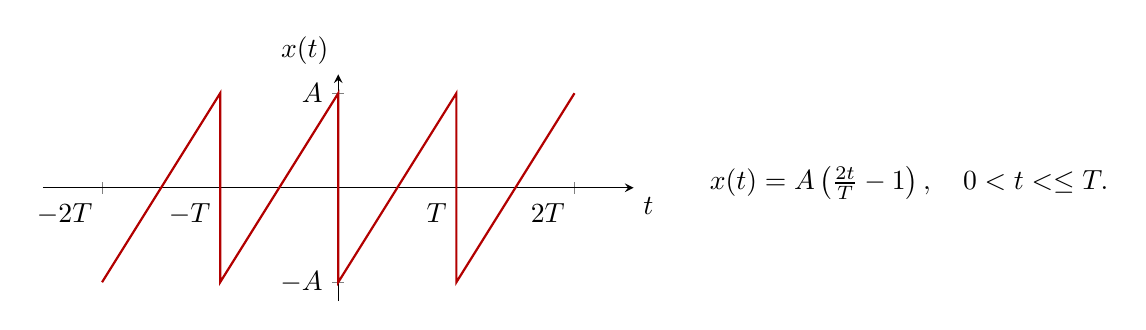
\begin{tikzpicture}[>=latex]
        \begin{axis}[
            x = 1.5cm,
            y = 0.6cm,
            domain=-2:2,
            no markers,
            axis x line=center,
            axis y line=center,
            xlabel style={below right},
            ylabel style={above left},
            xlabel = {$t$},
            ylabel = {$x(t)$},
            ytick={-2, 2},
            yticklabels = {$-A$, $A$},
            xtick={-2,-1, 0, 1, 2},
            xticklabels = {$-2T$, $-T$, 0, $T$, $2T$},
            xticklabel style={below left},
            xmin=-2.5,
            xmax=2.5,
            ymin=-2.4,
            ymax=2.4
            ]
            \addplot[thick, color=red!70!black] coordinates {(-2, -2) (-1, 2) (-1, -2)
            (0,2) (0, -2) (1, 2) (1,-2) (2, 2)};
        \end{axis}
        \pause
        \node at (11,1.5) {$x(t) = A\left(\frac{2t}{T} - 1\right), \quad 0 < t < \leq T.$};
    \end{tikzpicture}
\end{frame}

\begin{frame}
Example: Computing $a_k$
    \begin{columns}
        \begin{column}{0.5\textwidth}
            \begin{align*}
                a_0 &= \frac{1}{T}\int_T x(t)dt\\
                &= \frac{A}{T}\int_0^T \left(\frac{2t}{T} - 1\right)dt\\
                &= \left[\frac{2t^2}{2T}-t\right]_0^T\\
                &= 0
            \end{align*}
            \pause
            \begin{align*}
                a_k &= \frac{1}{T}\int_T x(t)e^{-jk\omega_0 t}dt\\
                    &= \frac{A}{T}\int_0^T \tikzmark{u}\left(\frac{2t}{T} - 1\right) \tikzmark{dv}e^{-jk\omega_0 t}dt\\
                    &=  \frac{A}{T}\left\{ \left[ \left(\frac{2t}{T}-1\right)\frac{e^{-jk\omega_0 t}}{-jk\omega_0}\right]_0^T -  \left[\frac{e^{-jk\omega_0 t}}{-jk\omega_0}\frac{2}{T}\right]_0^T\right\}
            \end{align*}
            \begin{tikzpicture}[
              remember picture,
              overlay,
              expl/.style={draw=orange,fill=orange!30, text centered},
              arrow/.style={red!80!black,ultra thick,->,>=latex}
            ]
            \node<2->[expl,text width=0.8cm]
              (u)
              at ([xshift=4.8ex, yshift=5ex]{pic cs:u})
              {$u$};
            \node<2->[expl, text width=1.2cm]
              (dv)
              at ([xshift=4.8ex, yshift=4ex]{pic cs:dv})
              {$dv$};
            \end{tikzpicture}
        \end{column}
        \begin{column}{0.5\textwidth}
        \pause
            \begin{align*}
                a_k &= \frac{A}{T}\left\{
                 \left[ \left(2-1\right)\frac{e^{-jk\tikzmark{omega0t}\omega_0 T}}{-jk\omega_0} - \frac{(-1)}{-jk\omega_0}\right]\right.\\
                 &-  \left.\frac{2}{-jk\omega_0T}\left[e^{-jk\omega_0T} - 1\right]
                 \right\}\\
                 &= \frac{A}{T}\left\{ \frac{-2}{jk\omega_0} \right\}\\
                 &= \frac{Aj}{\pi k}.
            \end{align*}
            \begin{tikzpicture}[remember picture, overlay]
            \node<3->[draw=orange,fill=orange!30,text width=1.2cm]
              (u)
              at ([xshift=2.4ex, yshift=6ex]{pic cs:omega0t})
              {$\omega_0T = 2\pi$};
            \end{tikzpicture}
            \pause
            \begin{equation*}
                a_k = \begin{cases} 0, & k = 0,\\ \frac{Aj}{\pi k},& k \neq 0.\\
                \end{cases}
            \end{equation*}
        \end{column}
    \end{columns}
\end{frame}


\begin{frame}
Example: Computing the Average Power
    \begin{align*}
        \frac{1}{T}\int_T |x(t)|^2dt &= \frac{A^2}{T}\int_0^T  \left(\frac{2t}{T} - 1\right)^2dt\\
        &=  \frac{A^2}{T}\int_0^T  \left[ \frac{4t^2}{T^2} - 4\frac{t}{T} + 1\right]\\
        &=  \frac{A^2}{T}\int_0^T  \left[ \frac{4t^3}{3T^2} - 4\frac{t^2}{2T} + t\right]\\
        &=  \frac{A^2}{T}\left[ \frac{4}{3T} - 2T + T\right]_0^T\\
        &= \frac{A^2}{3}
    \end{align*}
\end{frame}



\begin{frame}
Example: Verifying Parseval's relation
    \begin{align*}
        \sum_{k=-\infty}^{\infty}|a_k|^2 &= \sum_{k \neq 0}\left|\frac{Aj}{\pi k} \right|^2\\
        &=  2\frac{A^2}{\pi^2}\sum_{k \neq 1}^{\infty}\frac{1}{ k^2}\\
        &= 2\frac{A^2}{\pi^2}\frac{\pi^2}{6}\\
        &= \frac{A^2}{3}
    \end{align*}
    \begin{tikzpicture}[
      remember picture,
      overlay,
      expl/.style={draw=orange,fill=orange!30, text centered},
    ]
    \node[expl] at (12,4) {$\sum_{k=1}^{\infty}\frac{1}{k^2} = \frac{\pi^2}{6}$};
    \end{tikzpicture}
\end{frame}




\begin{frame}[plain]{Other Forms of Fourier Series}
    \begin{columns}
        \column{0.5\textwidth}
    Complex Exponential Fourier Series
            \begin{equation}
                \begin{aligned}
                    x(t) &= \sum_{k=-\infty}^{+\infty}a_k e^{jk\omega_0 t}\\
                    a_k &= \frac{1}{T} \int_{T}x(t)e^{-jk\omega_0 t}dt
                    %\omega_0 &= \frac{2\pi}{T}
                \end{aligned}
            \end{equation}
        \column{0.5\textwidth}
    Trigonometric Fourier Series
            \begin{equation}
                \begin{aligned}
                    x(t) &= A_0 + 2\sum_{k=1}^{+\infty} A_k\cos k\omega_0 t + B_k\sin k\omega_0 t\\
                    A_k &= \frac{1}{T} \int_{T}x(t)A_k\cos k\omega_0 t dt\\
                    B_k &= \frac{1}{T} \int_{T}x(t)A_k\sin k\omega_0 t dt
                    %\omega_0 &= \frac{2\pi}{T}
                \end{aligned}
            \end{equation}
    \end{columns}

    \begin{columns}
        \column{0.5\textwidth}
    Harmonic Form  Fourier Series (for Real $x(t)$)
            \begin{equation}
                \begin{aligned}
                    x(t) &= C_0 + 2\sum_{k=1}^{+\infty} C_k\cos (k\omega_0 t - \theta_k)\\
                    C_0 &= A_0\\
                    C_k &= \sqrt{A_k^2 + B_k^2} \quad                     \theta_k = \tan^{-1}\left(\frac{B_k}{A_k}\right)
                \end{aligned}
            \end{equation}
        \column{0.5\textwidth}
    Relationship
        \begin{equation}
            \begin{aligned}
                A_0 &= a_0\\
                A_k &= \frac{a_k + a_{-k}}{2}\\
                B_k &= j\frac{a_k - a_{-k}}{2}\\
                \omega_0 &= \frac{2\pi}{T}
            \end{aligned}
        \end{equation}
    \end{columns}




\end{frame}


\subsection{Convergence of Fourier Series}

\begin{frame}{Convergence of Fourier Series}
    Fourier series representation:
    \begin{equation*}
            x(t) = \sum_{k=-\infty}^{+\infty}a_k e^{jk\omega_0 t}
    \end{equation*}
    Consider the \alert{finite} series of the form
    \begin{equation*}
            x_N(t) = \sum_{k=-N}^{+N}a_k e^{jk\omega_0 t}
    \end{equation*}
    Let $e_N(t)$ denote the approximation error, that is,
    \begin{equation*}
            e_N(t) = x(t) - x_N(t) = x(t) - \sum_{k=-N}^{+N}a_k e^{jk\omega_0 t}
    \end{equation*}
    A quantitative measure of approximation error is
    \begin{equation*}
        E_N = \int_T \left|e_N(t)\right|^2 dt
    \end{equation*}


    \begin{tikzpicture}[remember picture,overlay]
    \node[draw=blue!50, fill=blue!20, inner sep=2pt,outer sep=2pt, rounded corners=0.1cm, anchor=south east, yshift=6cm, xshift=-1cm, text width=5cm]  at (current page.south east) {
        FS synthesis and analysis equations:
        \begin{equation*}
            \begin{aligned}
                x(t) &= \sum_{k=-\infty}^{+\infty}a_k e^{jk\omega_0 t}\\
                a_k &= \frac{1}{T} \int_{T}x(t)e^{-jk\omega_0 t}dt
            \end{aligned}
        \end{equation*}
    } ;
    \end{tikzpicture}
\end{frame}


\begin{frame}{Convergence of Fourier Series}
    \begin{itemize}[<+->]
        \item If $x(t)$ has a Fourier series representation, then the limit of $E_N$ as $N \rightarrow \infty$ is zero.
        \item If $x(t)$ does not have a Fourier series representation, then the integral that computes $a_k$ may diverge. Moreover, even if all of the coefficients $a_k$ obtained  are finite, when these coefficients are substituted into the synthesis equation, the resulting infinite series may not converge to the original signal $x(t)$.
        \item Fortunately, there are no convergence difficulties for large classes of periodic signals, continuous and discontinuous.
    \end{itemize}


\end{frame}


\begin{frame}{Finite-Energy Convergence Criterion}
    One class of periodic signals that are representable through the Fourier series is those signals which have finite energy over a single period:
    \begin{equation}
        \int_T \left|x(t)\right|^2 dt < \infty
    \end{equation}

    \begin{itemize}[<+->]
        \item In this case coefficients $a_k$ are finite.
        \item As $N\rightarrow \infty$, $E_N \rightarrow 0$.
        \item This \alert{does not imply that the signal $x(t)$ and its Fourier series representation are equal at every value of $t$}. What it does say is that there is no energy in their difference.
        \item However, since physical systems respond to signal energy, from this perspective $x(t)$ and its Fourier series representation are indistinguishable.
    \end{itemize}
\end{frame}

\begin{frame}{Alternative Conditions (Dirichlet Conditions)}

    Dirichlet conditions guarantee that $x(t)$ \alert{equals} its Fourier series representation, except at isolated values of $t$ for which $x(t)$ is discontinuous. At these values, the infinite series converges to the average of the values on either side of the discontinuity.\\[10pt]

    \noindent {\bf Condition 1}

    Over any period, $x(t)$ must be absolutely integrable
    \begin{equation}
        \int_T \left|x(t)\right| dt < \infty.
    \end{equation}
    This guarantees that $a_k$s are finite. \\[10pt]


    \noindent {\bf Condition 2}


    In any finite interval of time, $x(t)$ is of bounded variation; that is, there are no more than a finite number of maxima and minima during any single period of the signal. \\[10pt]


    \noindent {\bf Condition 3}

    In any finite interval of time, there are only a finite number of discontinuities. Furthermore, each of these discontinuities is finite.

\end{frame}

\begin{frame}{Examples of Functions that Violate Dirichlet Conditions}
    \begin{itemize}
        \item [Cond. 1] The periodic signal with period 1 with one period defined as
        \begin{equation*}
            x(t) = \frac{1}{t}, \quad 0 < t\leq 1.
        \end{equation*}
        \item [Cond. 2] The periodic signal with period 1 with one period defined as
        \begin{equation*}
            x(t) = \sin\left(\frac{2\pi}{t}\right), \quad 0 < t\leq 1.
        \end{equation*}
        For this
        \begin{equation*}
            \int_0^1 \left|x(t)\right| dt < 1
        \end{equation*}
        The function has, however, an infinite number of maxima and minima in the interval.
        \item [Cond. 3] The signal, of period T = 8, is composed of an infinite number of sections, each of which is half the height and half the width of the previous section. Thus, the area under one period of the function is clearly less than 8. However, there are an infinite number of discontinuities in each period, thereby violating Condition 3.
    \end{itemize}
\end{frame} 